% begin module continuity-ex1
\begin{frame}
\begin{example}[Example 1, p. 113]
The picture below shows a graph of a function $f$.  \alert<handout:0 |2-3>{At which numbers is $f$ discontinuous?}  \alert<handout:0 |4->{Why?}
\begin{columns}[c]
\column{.5\textwidth}
\ 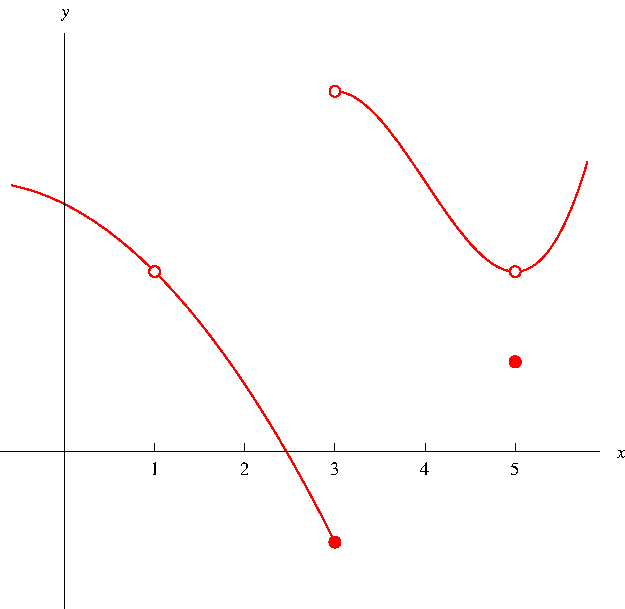
\includegraphics[height=4.5cm]{continuity/pictures/02-05-ex1.pdf}%
\column{.5\textwidth}
\begin{itemize}
\item<3->  Discontinuous at $1$:
\item<4->  \alert<handout:0 |5-6>{$\lim_{x\rightarrow 1}f(x)$ \uncover<6->{exists.}}
\item<4->  \alert<handout:0 |7-8>{$f(1)$ \uncover<8->{doesn't exist.}}
\item<3->  Discontinuous at $3$:
\item<4->  \alert<handout:0 |9-10>{$f(3)$ \uncover<10->{exists.}}
\item<4->  \alert<handout:0 |11-12>{$\lim_{x\rightarrow 3}f(x)$ \uncover<12->{doesn't exist.}}
\item<3->  Discontinuous at $5$:
\item<4->  \alert<handout:0 |13-14>{$f(5)$ \uncover<14->{exists.}}
\item<4->  \alert<handout:0 |15-16>{$\lim_{x\rightarrow 5}f(x)$ \uncover<16->{exists.}}
\item<17-| alert@17>  $\lim_{x\rightarrow 5}f(x) \neq f(5)$.
\end{itemize}
\end{columns}
\end{example}
\end{frame}
% end module continuity-ex1
